\documentclass{book}
\usepackage[spanish]{babel}
\usepackage[a4paper]{geometry}
\geometry{top=2.5cm, bottom=2.5cm, left=3cm, right=2cm}
\renewcommand{\baselinestretch}{1.5}
\usepackage{fontspec}
\setromanfont{Carlito}
\usepackage{xcolor}
\usepackage{titlesec}
\usepackage{ragged2e}
\usepackage{hyperref}
\usepackage{float}
\usepackage{graphicx}
%% COSO DE HACER GLOSARIOS
%\usepackage{glossaries}
%\newacronym{es}{E/s}{entrada/salida}
%\makeglossaries
\usepackage{fancyhdr} % paqauete para el estilo del page numering y de todo un poco



\cfoot{  \textbf{\thepage} } 


%desde aqui es de alex
\definecolor{gray75}{gray}{0.75}
\newcommand{\hsp}{\hspace{5pt}}
\titleformat{\chapter}[hang]{\Large\bfseries}{\Large\thechapter.\hsp}{0pt}{\Large\bfseries}
\titlespacing*{\chapter}{0pt}{-30pt}{0pt}

\newcommand{\chapterA}[1]{
    \chapter{#1}
    \vspace{-0.5ex}%
    \noindent \rule{\textwidth}{0.3pt}
}
%hasta aqui es el chapter de alex
\pagestyle{plain}

\title{Trabajo resumen}


\begin{document}

\frontmatter


\begin{titlepage}
\begin{center}

\vspace*{6\baselineskip} % PARA BAJAR X LÍNEAS

{\scshape\Huge \textbf{Unidad 1: Explotación de Sistemas Informáticos } \par}

\vspace{3cm}

{\bfseries\LARGE I.E.S. AZARQUIEL }

\vspace{1cm}

{\scshape\Large  \textbf{Grado Superior de Desarrollo de Aplicaciones Web}\par}


{\Large \textbf{Alumna:} \par}
{\Large   \textbf{Alicia Sánchez Lorente} \par}
{\Large  \textbf{Profesor:} \par}
{\Large  \textbf {Carlos Vicente Charco}\par}
\vfill
{\Large  \textbf{16 de octubre de 2022} \par}

\end{center}
\end{titlepage}
 
\shipout\null

\newpage

\begin{center}
    \textbf{\LARGE Resumen}
    \end{center}

\begin{large}

En el siguiente trabajo presentaré una síntesis de los contenidos vistos hasta ahora durante el curso. Me enfocaré no tanto en explicar lo dado, como en realizar un bosquejo que pueda servirme como repaso general de forma que de un solo vistazo pueda repasar los principales contenidos del tema a la hora de estudiar.

Antes de empezar me gustaría señalar las herramientas utilizadas para llevar este trabajo a cabo. Al contrario que mis compañeros, que han utilizado LibreOffice o el Word, finalmente me decanté por hacerlo en \textit{Overleaf}. Siempre tuve entendido que este editor colaborativo de \LaTeX\ es una herramienta profesional de edición de texto bastante utilizada a la hora de publicar libros o artículos científicos, especialmente en el campo de la informática. Cierto es que me ha costado un par de tardes tarde entera hacer la plantilla, pero viendo el resultado, ha valido la pena completamente.

Para el contenido de esta síntesis me he servido de los apuntes de clase como base, pero la verdad es que aunque mi primera intención es realizar el trabajo y obtener buena nota, principalmente me interesa mejorar mi capacidad de síntesis, estudiar (pues no puedo resumir lo que no comprendo) y realizar el bosquejo a partir del cual partir a la hora de estudiar para el examen.

\end{large}




%\maketitle Para poner de nuevo el titulo, creo?


    
\renewcommand\contentsname{\begin{center}Índice\end{center}}
\renewcommand{\listfigurename}{\begin{center}Índice de figuras\end{center}}
\renewcommand{\listtablename}{\begin{center}Índice de tablas\end{center}}

\tableofcontents

\let \cleardoublepage \clearpage


\listoffigures
\addcontentsline{toc}{chapter}{Índice de figuras}

\let \cleardoublepage \clearpage

\listoftables
\addcontentsline{toc}{chapter}{Índice de tablas}

\mainmatter

\chapter{Introducción}

\begin{large}

A continuación se tratarán  los principales contenidos del tema de forma resumida, ordenada y precisa.

He organizado este trabajo de la primera unidad, titulada ''Explotación de sistemas informáticos'', en puntos principales y subpuntos. No quise introducir más subpuntos porque mi objetivo es un trabajo claro y sencillo. Por esta razón no he introducido más definiciones de las necesarias y solo he aclarado los conceptos clave y aquellos más importantes.

Con respecto a la estructura del trabajo, seguiré el orden de clase alterando algunos subpuntos por preferencia personal para una mejor comprensión de los temas. En primer lugar introduciré los sistemas informáticos, continuaré con los elementos funcionales de un ordenador digital, el microprocesador, la Unidad de Memoria, la placa base, la GPU y los buses y periféricos, para terminar con una conclusión.

\end{large}

\section{\textbf{Temario}}\label{sec:Temario}

\subsection {\textbf{Los sistemas informáticos}}

\begin{large}

Un sistema informático (SI) es el sistema cuya función es recoger datos, procesarlos y transmitir información. Esta formado por el \textit{software} (la parte no tangible), el \textit{hardware} (la parte tangible) y el componente humano.

La información que le llega es procesada mediante sistemas de numeración, de los que existen dos tipos: no posicionales y posicionales. 
Entre estos últimos a su vez podemos distinguir entre el sistema de numeración binario, octal, hexadecimal y decimal.

\end{large}

\subsection {\textbf {Elementos funcionales de un ordenador digital}}

\begin{large}

Los ordenadores están compuestos por: elementos eléctricos, puertas lógicas, circuitos integrados y los ya nombrados sistemas de numeración.

La arquitectura de un ordenador determina el comportamiento funcional, estableciéndose unos componentes encargados de realizar operaciones siguiendo unas pautas concretas. La más utilizada es la de Von Neumann [Figura 2.1]

Entre las unidades funcionales del ordenador digital encontramos la unidad de entrada/salida (E/S) \footnote {\normalsize Para saber más ver Ruiz Ortiz, J.M., (2011) \textit{Tema 8: Organización de la Entrada/Salida}, Universidad Complutense de Madrid}, la unidad de memoria \footnote {\normalsize Para saber más ver Ruiz Ortiz, J.M., (2011) \textit{Tema 5: Organización de la memoria: memoria principal}, Universidad Complutense de Madrid}, la unidad del proceso, formada a su vez por la Unidad Aritmético-Lógica (ALU) y la unidad de control (UC)\footnote {\normalsize Para saber más ver ROCA, J.(2022), "¿Cómo se gestiona a sí misma una CPU? Así funciona la unidad de control", \textit{HardZone}.}. 

\end{large}

\subsection {\textbf {Microprocesador}}

\begin{large}

En este apartado nos centramos en la ya nombrada CPU. La podemos definir brevemente como el ``cerebro'' de un sistema informático ya que controla el \textit{hardware},envía instrucciones y realiza los cálculos \footnote {\normalsize \textit{¿Qué es un microprocesador? ¿Cuál es su función?}, PC Componentes, https://www.pccomponentes.com/que-es-un-microprocesador-cual-es-su-funcion}.

Como ya hemos dicho, está formada por: 

\begin{itemize}

    \item La ALU, encargada de operaciones binarias simples y formada por el bus, R. en a y R. en b, el acumulador, lo registros de estado y el circuito operacional, que a su vez está integrado por el circuito semisumador, el sumador, el restador y el semirestador.
    
    \item  Con respecto a la UC, se encarga de dar las órdenes a los dispositivos del ordenador. Está formado por el registro contador de programa (CP), el Registro de Instrucción (RI),el decodificador, el reloj y el secuenciador [Figura 2.2]. 
    

\end{itemize}

Para llevar a cabo su tarea se dan cuatro fases con un total de 7 pasos % BUSCAR CITA

Conociendo ya su función en un ordenador, veamos las características principales de la CPU: la frecuencia de reloj (mide los ciclos por segundo), el número de hilos de procesamiento (generalmente, cuantos más tenga, más tareas podrá ejecutar a la vez) y el IPC (Instrucciones Por Ciclo)

Además, al configurar la CPU se ha de tener en cuenta el juego de instrucciones adecuado, temiendo presente los tipos de instrucciones: de transferencia de información, aritmético-lógicas y de desplazamiento, de transferencia de control y misceláneas. Dependiendo de su complejidad, puede contar con dos tipos de estructuras: CISC (para instrucciones complejas) y RISC (para instrucciones simples).

Además, la CPU necesita contar con determinados componentes para funcionar: memoria caché (L1, L2, L3), coprocesador matemático (FPU), unidad de gestión de memoria (MMU) y el encapsulado.

\end{large}

\subsection {\textbf{Unidad de Memoria}}

\begin{large}


Existe una jerarquía de memoria con distintos niveles: nivel 0, la CPU; nivel 1, la memoria caché; nivel 2, la memoria RAM; nivel 3, discos magnéticos y unidades de estado sólido; y  nivel 4, dispositivos de almacenamiento masivo \footnote {\normalsize M. A. Orenga y G. E. Manonellas, \textit{Sistema de memoria}, Estructura de computadores, Universitat Oberta de Catalunya http://cv.uoc.edu/annotation/8255a8c320f60c2bfd6c9f2ce11b2e7f/619469/PID\_00218275/PID\_00218275.html}

Aquí podemos distinguir entre memoria SRAM (consumen menos energía y su diseño es más complicado) y la DRAM (consumen mas energía, pero su diseño es más sencillo).

Existen, por otra parte, algunas memorias únicamente de lectura: ROM PROM, EPROM y EEPROM.

Entre sus características, podemos señalar la velocidad o frecuencia, la capacidad, el tiempo de acceso y la latencia CAS.

La memoria RAM envía la información al procesador mediante los canales de memoria. Pueden tener uno o más de uno (Dual Channel). Éste puede transferir dos módulos de memoria simultáneamente, pero para que funcione todos los módulos de la memoria RAM deben ser iguales.
Además existe el Quad channel, que habilita cuatro canales, pero es más profesional.

\end{large}

\subsection {\textbf {La placa base}}

\begin{large}

Este componente se encarga de interconectar los componentes de un ordenador. Para ello está formado por conectores: el socket o zócalo, donde se conecta la CPU (puede ser de dos tipos: ZIP y LGA), Zócalo DIMM (entre 2 o 4 ranuras para las memorias RAM) y las ranuras de expansión (para conectar la tarjeta gráfica, la de sonido y la de red).

Hay además varios tipos de formas de placa base: EATX, ATX, micro-ATX y mini-ITXv \footnote{\normalsize García García-Doncel, J.,(24 de noviembre de 2021), \textit{La placa base}, Data Science, Sitio web para aprender Data Science, https://dat-science.com/la-placa-base/}.

Otro componente que destacan dentro de la placa es el \textit{chipset}, divido en dos chips: el  \textit{Northbridge} y el \textit{Southbridge}. El primero, conecta la placa con el miroprocesador, la tarjeta gráfica y los módulos de memoria; el segundo, sin embargo, da soporte LAN, conecta con los puertos PCIe, USB y SATA. El \textit{Northbridge} ha desaparecido de la placa porque se incorpora el procesador. Por otra parte el \textit{Southbridge} ha sido sustituido por el PCH \textit{Platform Hub Controller}.

En la placa base encontramos también otro chip denominado la  \textit{BIOS}, encargado de verificar que todos los sistemas funcionan al arrancar el equipo, mediante el \textit{software} de verificación (\textit{Power-On Self Test}), además de dar soporte a ciertos dispositivos de entrada y salida. 

\end{large}

\subsection{\textbf{La GPU o Tarjeta Gráfica}}

\begin{large}
Este componente se encarga de "traducir" la información del microprocesador para mostrarla en el monitor.
Se pueden colocar en el PCIe, el procesador o en la placa base y tiene su propia memoria incorporada (GDDR).

Los parámetros de este componente son: la resolución, la profundidad del color, la tasa de refresco.

\end{large}

\subsection{\textbf{Buses y periféricos}}
\begin{large}
Un bus es el ''camino por el que circula la información". Pueden ser datos, señales o instrucciones. Existen varios tipos de buses clasificados de 0 a 5. Serían buses por ejemplo los buses ISA, el cable que conecta a la impresora o los cables de red Ethernet. Además cuentan con una serie de factores que determinan su capacidad de transmisión, como el ancho o la frecuencia.

Un periférico permite la conexión del ordenador con el exterior. Hay tres tipos: de entrada (ej. ratón, micrófono), de salida (ej. altavoz o impresora), de entrada/salida (ej. pendrives).

Algunos ejemplos de periféricos son: el teclado, el ratón, el escáner, la impresora, el monitor.

Para conectar el dispositivo al ordenador hemos de tener en cuenta la interfaz de conexión, como a través de: VGA, DVI, Displayport,HDMI, USB, Thunderbolt, FireWire,Jack 3.5mm, Ethernet, Puerto serie, puerto paralelo, puerto PS/2, puerto MIDI (Musical Instrument Digital Interface). [Figura 3.1]

\end{large}

\subsection{\textbf{Conclusión}}

\begin{large}

Hacer un trabajo de estas características no ha sido muy novedoso para mi ya que en la universidad he tenido que hacer bastantes así. Sin embargo me ha resultado difícil resumir contenidos porque, como señalé en la introducción, mi objetivo con este trabajo es realizar un resumen del que partir para estudiar. Considero, además, haberlo conseguido. Principalmente estoy satisfecha por lo que he aprendido en el proceso, tanto sobre la asignatura como sobre Overleaf, a cuyo código se puede acceder  \href{https://github.com/AliSanLo/DAW/tree/main/SISIN}{clicando aquí} o en este enlace \url {https://github.com/AliSanLo/DAW/tree/main/SISIN} , de mi GitHub. Espero poder seguir avanzando para seguir aplicando todo lo aprendido a lo largo del Grado y mi carrera profesional y laboral. 



\end{large}


\chapter{Anexo de imágenes}

\begin{figure}[H]
    \centering
    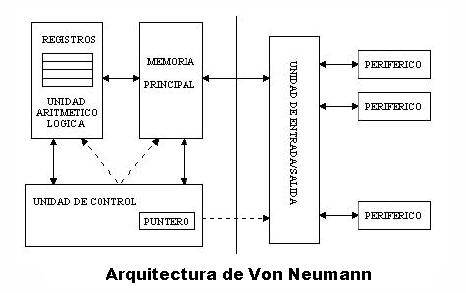
\includegraphics[width=1\textwidth]{figures/Von_Neumann.png}
    \caption{ \Centering Diagrama  de la arquitectura Von Neumann} 
    
    \textit{Arquitectura de Von Neumann}, Jesus's website, \url{https://sites.google.com/site/jesusswebsite/unidad-2-estructura-y-componentes-de-una-computadora/estructura-de-von-neumann}
    \label{fig:arq_vn}
\end{figure}


\begin{figure}[H]
    \centering
    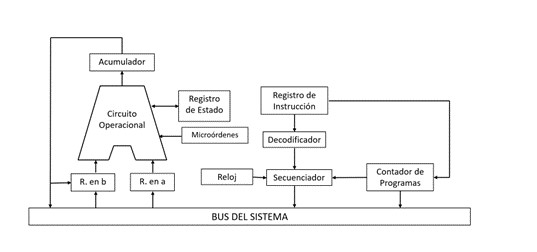
\includegraphics[width=1\textwidth]{figures/ALU .jpg}
    \caption{ Esquema representativo de la ALU y la UC}
    
    De elaboración propia
    \label{fig:ALU}
\end{figure}


\chapter{Anexo de tablas}

\begin{table}[H]
\begin{tabular}{|l|l|l|l|}
\hline
\textbf{DISPOSITIVO} & \textbf{INTERFAZ DE CONEXION}                                                                                  & \textbf{DISPOSITIVO}            & \textbf{INTERFAZ DE CONEXIÓN}                                                                                              \\ \hline
\textbf{Ratón}       & \begin{tabular}[c]{@{}l@{}}USB\\ PS2\end{tabular}                                                              & \textbf{Cámara de fotos}        & \begin{tabular}[c]{@{}l@{}}HDMI Mini\\ HDMI Micro\\ HDMI\end{tabular}                                                      \\ \hline
\textbf{Teclado}     & USB                                                                                                            & \textbf{Pen Drive}              & USB                                                                                                                        \\ \hline
\textbf{Monitor}     & \begin{tabular}[c]{@{}l@{}}VGA\\ DVI\\ HDMI\\ DisplayPort\end{tabular}                                         & \textbf{Tableta digitalizadora} & \begin{tabular}[c]{@{}l@{}}USB \\ Bluetooth\end{tabular}                                                                   \\ \hline
\textbf{Altavoces}   & \begin{tabular}[c]{@{}l@{}}ADAT\\ FireWire\\ USB\\ TS\\ TRS\\ S/PDIF-RCA\\ XLR\\ BNC\\ RCA\\ MIDI\end{tabular} & \textbf{Webcam}                 & \begin{tabular}[c]{@{}l@{}}Camera Link\\ USB 2.0\\ IEEE 1349a\\ IEEE 1394(FireWire)\\ GigE (Gigabit Ethernet)\end{tabular} \\ \hline
\textbf{Impresora}   & \begin{tabular}[c]{@{}l@{}}COM\\ USB\\ Ehternet\\ Centronic\end{tabular}                                       & \textbf{Proyector}              & \begin{tabular}[c]{@{}l@{}}Puerto Audio Out\\ Puerto Monitor Out\\ Conector Display Port\\ Puerto HDMI\end{tabular}        \\ \hline
\textbf{Auriculares} & Minijack                                                                                                       & \textbf{Escáner}                & \begin{tabular}[c]{@{}l@{}}USB\\ FireWire\\ SCSI\\ Puerto Paralelo\end{tabular}                                            \\ \hline
\end{tabular}
\caption{Interfaz de conexión de algunos periféricos}
\label{tab:Interfaz.de.conexión}
\end{table}

\chapter{Bibliografía y webgrafía}

\begin{large}

\begin{itemize}

    \item Ruiz Ortiz, J.M., (2011) \textit{Tema 8: Organización de la Entrada/Salida}, Universidad Complutense de Madrid. Apuntes de la asignatura Estructura de Computadores de la Facultad de Informática. 
    
    \url{http://www.fdi.ucm.es/profesor/jjruz/web2/temas/ec8.pdf }
    
    \item Ruiz Ortiz, J.M., (2011) \textit{Tema 5: Organización de la memoria: memoria principal}, Universidad Complutense de Madrid. Apuntes de la asignatura Estructura de Computadores de la Facultad de Informática. 
    
    \url{http://www.fdi.ucm.es/profesor/jjruz/WEB2/Temas/EC5.pdf}
    
    \item ROCA, J.(2022), "¿Cómo se gestiona a sí misma una CPU? Así funciona la unidad de control", \textit{HardZone}
    
    \url{https://hardzone.es/reportajes/que-es/unidad-control/}
    
    \item García García-Doncel, J.,(24 de noviembre de 2021), \textit{La placa base}, Data Science, Sitio web para aprender Data Science, \url{https://dat-science.com/la-placa-base/}
    
    \item  Orenga, M. A. y  Manonellas, G. E., \textit{Sistema de memoria}, Estructura de computadores, Universitat Oberta de Catalunya 
    
    \url{http://cv.uoc.edu/annotation/8255a8c320f60c2bfd6c9f2ce11b2e7f/619469/PID\_00218275/PID\_00218275.html}
    
\end{itemize}

\end{large}

%\printglossary[title={Glosario}] % Mostrar el glosario, para meter una entrada nueva, meterla en glossary.tex y ponerla en el texto con \gls

\end{document}



